\chapter{Experiments}
\label{sec:experiments}

\section{Environment and Hardware}
\label{sec:experiments:environmentHardware}
The experiments were conducted on a SLURM cluster using nodes with \num{32} CPU cores, \SI{128}{\giga\byte} RAM and an Nvidia A-100 GPU with \SI{40}{\giga\byte} VRAM. The implementation is written in python 3.10.13. The data is stored in a SQLite database, the database schema can be found in Appendix~\ref{sec:appendix:databaseSchema}.

\section{Experimental Setup}
\label{sec:experiments:setup}

% TODO: introduction

\subsection{Attribute Sentence Generation}
\label{sec:experiments:setup:sentenceGeneration}
The synthetic dataset that consists of attribute sentences which describe a set of input texts is constructed by prompting an \acs{llm} in a two-step procedure. For this thesis, the open source model Llama 3.2 Instruct\footnote{\url{https://huggingface.co/meta-llama/Llama-3.2-3B-Instruct}}~(\cite{dubeyLlama3Herd2024}) with \num{3} billion parameters has been used. This model has state-of-the-art performance and is freely available, which provides the possibility to run the model directly on the server cluster. Additionally, it improves the reproducibility of the experiments because it is easier to use the exact same model later.
To improve the performance of the sentence generation, the library vLLM\footnote{\url{https://github.com/vllm-project/vllm}} was used to run the model.

The basis for the generation of the attribute sentences are \num{\numAnswersStyleVector} answers from the stack exchange dataset described in Section %~\ref{}. TODO:
For each of the answers, the model is prompted \num{\numPrompts} times to create descriptions of the text with the method presented in Section~\ref{sec:approach:attributeSentenceGeneration}.

For each of the resulting \num{\numStyleDescriptions}, the model is prompted again to convert the description into a list of sentences of the form \enquote{The author is \ldots} or \enquote{The author uses \ldots}. The output of the \ac{llm} is split into sentences using the Natural Language Toolkit\footnote{\url{https://www.nltk.org/}} library (\cite{birdNaturalLanguageProcessing2009}). The naive approach of splitting the sentences at the punctuation would not work as they could include punctuations with expressions such as \enquote{e.g.}.

The model is instructed to avoid negations and examples because they can lead to the sentences having a too dissimilar shape while conveying the same meaning. In addition to this constraint that is stated in the prompt, the final sentences are checked to not include the word \enquote{not}. If they do, they are skipped and not used for further computation. During the experiments, \num{\numSentencesWithNegations} sentences have been filtered because of this reason.

After the previous steps, \numStyleSentencesNotUniqueText{} attribute sentences have been produced. After taking into account only unique sentences, \numStyleSentencesText{} attribute sentences are left. Of these, \num{\numStyleSentencesStyle} sentences are style sentences, which means they have been produced by a style prompt, and \num{\numStyleSentencesKnowledge} are knowledge prompts.
% TODO: are style sentences + knowledge sentences = all sentences? if not, explain

\subsection{Clustering}
\label{sec:experiments:setup:clustering}
Although the number of sentences is reduced significantly by checking for exact duplicates, there are still lots of sentences that have basically the same meaning while being not exactly the same. This can lead to the problem that it would not be clear if an attribute sentence has rarely been used to describe the input texts or if the \ac{llm} has just a high syntactic variance in describe one concept.

The solution to this problem that this thesis is to cluster the sentences and use the clusters as attributes by using the sentence that is closest to the center as the representation for the cluster.
The first step for this procedure is to create an embedding of all sentences so they can be compared semantically. The SBERT model \textit{all-MiniLM-L12-v2}\footnote{\url{https://huggingface.co/sentence-transformers/all-MiniLM-L12-v2}} (\cite{reimersSentenceBERTSentenceEmbeddings2019}) was used to create the embeddings.

For the following steps, the style and knowledge sentences have been processed separately to ensure the resulting clusters are either style or knowledge clusters.
The clustering algorithm first computes a radius neighbor graph of all sentences. All sentences that have a cosine similarity higher than \num{\minCosineSimilarity} are considered to be in the same cluster. Subsequently, the clusters are sorted by size and inspected from largest to smallest. If a sentence is included in one cluster, it is removed from all smaller ones. It is important to note that there is no minimum size for a cluster; if a sentence has no neighbors or every one of them is already part of a larger cluster, then the cluster size is one.

% TODO: why 0.85 min similarity?

At this point, there \num{\numClusters} clusters, \num{\numClustersStyle} of which are style clusters and \num{\numClustersKnowledge} are knowledge clusters. The size of the complete synthetic dataset can be found in Table~\ref{table:syntheticDataset}.

\begin{table}[ht]
  \begin{center}
    \begin{tabular}{lS[table-format=7.0]}
      \toprule
                   & {Number of data points} \\ \midrule
      Answers      & \numAnswersStyleVector  \\
      Prompts      & \numPrompts             \\
      Descriptions & \numStyleDescriptions   \\
      Sentences    & \numStyleSentences      \\
      Clusters     & \numClusters            \\ \bottomrule
    \end{tabular}
  \end{center}
  \caption{The size of the synthetic dataset created for this thesis. The answers are the group-specific input texts that are taken from the stack exchange dataset (see Section~\ref{sec:datasets:stackex}). For each answer and prompt, the \ac{llm} is prompted to create the style and knowledge descriptions. The descriptions are converted to attribute sentences by prompting the model again. Finally, the sentences are clustered together by the cosine similarity of their embeddings. The embeddings where produced with an SBERT model (\cite{reimersSentenceBERTSentenceEmbeddings2019}).}
  \label{table:syntheticDataset}
\end{table}

\subsection{Selecting the Attribute Vector Dimensions}
\label{sec:experiments:setup:selection}
The synthetic dataset resulting from the previous steps consists of \num{\numClusters} clusters which are the potential dimensions of the interpretable attribute vector. This vector however consists of \num{\styleVectorSize} dimensions as established by \citet{patelLearningInterpretableStyle2023}. Therefore, the best clusters have to be selected to be part of the attribute vector. This selection is carried out in multiple steps which are described in the following section and additionally shown in Figure~\ref{fig:clustering}.

\begin{figure}[ht]
  \begin{center}
    % \begin{tikzpicture}[
    % arrow tip
    >=Stealth,
    % box style
    box/.style={
        draw,
        rectangle,
        minimum width=50mm,
        minimum height=10mm,
        align=center
      },
    % dashed region style
    dashedbox/.style={
        draw,
        dashed,
        inner sep=6mm
      },
    % default distance between nodes
    node distance=8mm and 12mm
  ]

  % Top layer
  \node[box] (attrib) {Attribute Sentences};
  \node[box, below left=of attrib]  (stySent) {Style Sentences};
  \node[box, below right=of attrib] (knSent)  {Knowledge Sentences};

  % Clustering step
  \node[box, below=of $(stySent)!0.5!(knSent)$] (cluster)
  {Clustering by Cosine Similarity};

  % Resulting clusters
  \node[box, below left=of cluster]  (styCl) {Style Clusters};
  \node[box, below right=of cluster] (knCl)  {Knowledge Clusters};

  % Three sequential steps
  \node[box, below=of $(styCl)!0.5!(knCl)$] (step1)
  {used in maximum number of groups\\minimum usages};
  \node[box, below=of step1] (step2)
  {clusters with a minimum distance to each other};
  \node[box, below=of step2] (step3)
  {clusters with largest difference in agreement levels};

  % Dashed box around those three steps
  \node[dashedbox, fit=(step1)(step2)(step3)] {};

  % Final attribute-vector block
  \node[box, below=of step3] (attrVec) {
    \begin{tabular}{ccc}
      Targeted Style Attributes & Knowledge Attributes & Style Attributes
    \end{tabular}
    \\[2pt]
    \textbf{Attribute Vector}
  };

  % Arrows
  \draw[->] (attrib)  -- (stySent);
  \draw[->] (attrib)  -- (knSent);
  \draw[->] (stySent) -- (cluster);
  \draw[->] (knSent) -- (cluster);
  \draw[->] (cluster) -- (styCl);
  \draw[->] (cluster) -- (knCl);
  \draw[->] (styCl)    -- (step1);
  \draw[->] (knCl)     -- (step1);
  \draw[->] (step1)    -- (step2);
  \draw[->] (step2)    -- (step3);
  \draw[->] (step3)    -- (attrVec);
  \draw[->] (attrVec.west) .. controls +(-15mm,0) and +(-15mm,24mm) .. (stySent.west);

\end{tikzpicture}

    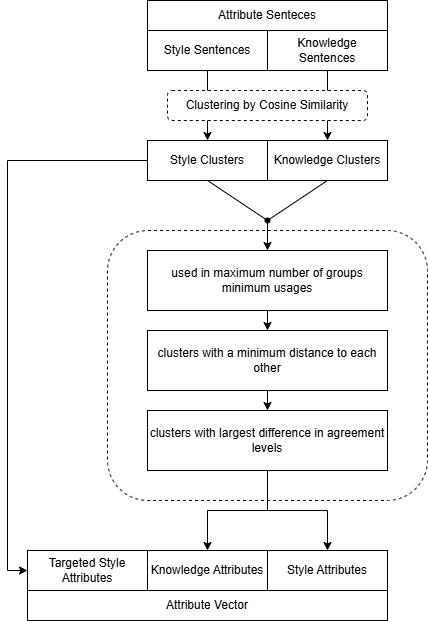
\includegraphics[width=9cm]{figures/clustering_diagram.png}
  \end{center}
  \caption{TODO:}
  \label{fig:clustering}
\end{figure}

\subsubsection{Selection of target attributes}
\label{sec:experiments:setup:selection:targetAttributes}
Following the work of \citet{patelLearningInterpretableStyle2023}, the first \num{\numTargetPrompts} dimensions of the attribute vector will be selected to correspond to the \num{\numTargetPrompts} target prompts, which were described in Section~\ref{sec:approach:attributeSentenceGeneration}.
This is done to ensure that the attribute vector has a robust foundation on some features that are manually selected for being relevant for stylistic research. The ability to automatically create most of the attribute vector is not significantly reduced since the target attributes only account for around \SI{10}{\percent} of its size.

These attributes are found by creating sentences of the form \enquote{The author uses <target>} and embedding them using the same embedding model that has been used to embed the attribute sentences, the all-MiniLM-L12-v2 model.
Afterward, for each sentence, the style cluster with the highest cosine similarity is found. This cluster is then one of the target attributes of the vector.

% TODO: write better?
The knowledge clusters are not taken into account during this selection. Since all style sentences that are produced by the targeted prompts can not be part of any knowledge cluster, any knowledge cluster that has a very high cosine similarity would be an unwanted cluster that should not be chosen at this point.

% TODO: compare to what patel et al. have done?

\subsubsection{Filtering out attributes that occur too frequently}
\label{sec:experiments:setup:selection:filteringOccurance}
An important characteristic of all attributes that are part of the attribute vector is that they are as meaningful as possible and help to distinguish between different groups. To ensure this requirement is met, attributes that describe texts of a too large portion of groups are removed. Based upon the work of \citet{patelLearningInterpretableStyle2023}, the maximum number of groups that can be described by an attribute cluster is \SI{60}{\percent}.

At the same time, the number of clusters that are taken into account for the next selection steps has to reduced because these steps have a quadratic memory requirement. To quickly reduce the number of clusters, the number of times the cluster was used to describe answers is taken into account. The required number of times used is increased until the resulting number of clusters is small enough. This way, the largest clusters that are not used to describe too many groups are used for the next steps.

To determine, how many times a cluster was used to describe an answer, each sentence is only counted once per answer. Multiple prompts could produce the same attribute sentence to describe an answer; counting all of them would however distort the number of usages of the clusters.

\subsubsection{Removing too similar Attributes}
\label{sec:experiments:setup:selection:removeSimilar}
To ensure that the attribute vector covers a wide range of attributes, it is important that the attributes do not cover too similar topics. This is achieved by ensuring that the clusters have a maximum cosine similarity of \num{\maxCosineSimilarity} to each other. This process works by ordering the clusters by occurrence, selecting them one after the other, and deleting all clusters that are too close to the ones that have already been selected.
The cosine similarity is computed between the embeddings of the attribute sentence that is closest to the center of the embedding.

% TODO: explanation why 0.7
\begin{itemize}
  \item patel et al have a maximum cosine similarity of 0.8, I have 0.7
  \item in this case, sentences that have a similarity higher than 0.85, they are in the same cluster
  \item a lower maximum similarity garantees a broader attribute vector
  \item when lower than 0.7, there are not enough attribute candidates
\end{itemize}

\subsubsection{Final Selection} % TODO: better name?
\label{sec:experiments:setup:selection:finalSelection}
The first \num{\numTargetPrompts} dimensions of the attribute vector are the target attributes that were selected in Section~\ref{sec:experiments:setup:selection:targetAttributes}. The next \num{\minNumKnowledgePrompts} dimensions are knowledge clusters, that is clusters of sentences that were produced by knowledge prompts. The rest of the dimensions are selected in this step to be the ones with the highest difference in agreement levels.

Difference in agreement levels means that the range between the answers that match the attribute really well and the ones that do not match is as big as possible. This further increases the probability that the attributes are well suited to distinguish between different answers and groups.

\lstinputlisting[language=Python, caption={Pseudo code for the final cluster selection step.}]{content/05-experiments/final-cluster-selection.py}

First, the similarity between all clusters that remain after the first selection steps is computed. Afterward, for each cluster and each answer, the average similarity to all other clusters that have been used to describe that answer is computed. The result is a rough estimation of the actual similarity between the current attribute sentence and the answer.

Subsequently, the range between the similarity of the most and least similar answers is computed, and the clusters with the highest difference are selected. With the process, the probability of attributes holding meaningful information to distinguish between different groups is increased.

\subsection{\acf{sfam}}
\label{sec:experiments:setup:sfam}

\begin{itemize}
  \item deberta-v3-base instead of \ldots{} used by \citet{patelLearningInterpretableStyle2023}
  \item sigmoid activation function to only produce values between 0 and 1
        \begin{itemize}
          \item \citet{patelLearningInterpretableStyle2023} used np.clip()
        \end{itemize}
\end{itemize}

\subsection{\acf{lisa}}
\label{sec:experiments:setup:lisa}

\begin{itemize}
  \item deberta-v3-large instead of \ldots{} used by \citet{patelLearningInterpretableStyle2023}
  \item sigmoid activation function to only produce values between 0 and 1
        \begin{itemize}
          \item \citet{patelLearningInterpretableStyle2023} used np.clip()
        \end{itemize}
\end{itemize}

\subsection{Steering}
\label{sec:experiments:setup:steering}

\begin{itemize}
  \item questions taken from \citet{petroni-etal-2021-kilt,rooeinKnowYourAudience2023}
\end{itemize}

\subsubsection{Activation Steering}
\label{sec:experiments:setup:steering:activation}

\begin{itemize}
  \item using layers in the middle based upon the research by \citet{konenStyleVectorsSteering2024,bogdanEmergentEffectsScaling2025}
\end{itemize}
